\documentclass{article} % For LaTeX2e
\usepackage{nips12submit_e,times,graphicx,amsmath,caption,subcaption,tikz,amsfonts}
%\documentstyle[nips12submit_09,times,art10]{article} % For LaTeX 2.09

\title{Graphical Model Control}

\author{
Craig Corcoran\\
Department of Computer Science\\
University of Texas at Austin\\
\texttt{ccor@cs.utexas.edu} \\
\And
Matthew Hausknecht\\
Department of Computer Science\\
University of Texas at Austin\\
\texttt{mhauskn@cs.utexas.edu} \\
}

\newcommand{\fix}{\marginpar{FIX}}
\newcommand{\new}{\marginpar{NEW}}

\nipsfinalcopy

\begin{document}
\maketitle

\begin{abstract}
  This paper explores a novel method of learning and control in Markov Decision Processes (MDPs). Most Reinforcement Learning algorithms employ variants of the Bellman equations to maximize expected long-term reward. In contrast, this work applies graphical model learning and inference to the problem of Inverse Reinforcement Learning (IRL), in which sample trajectories are provided as input to the agent and the goals is to 

to this work reduces finite timesteps in the MDP to Markov Random Fields. Inference and 
\end{abstract}

\section{Background}
A Markov Decision Process is a discrete time stochastic process where a decision making agent is required at each time step choose an action $a$ given its current state $s$. Formally an MDP is defined as a 4-tuple $\{S,A,P,R\}$ where $S$ is a finite set of states, $A$ is a finite set of actions, $P_a(s,s')$ is the probability that taking action $a$ in state $s$ at time $t$ will lead to state $s'$ at time $t+1$, and $R_a(s,s')$ is the immediate reward received after transition from state $s$ to state $s'$.

To solve an MDP, the challenge is to find a policy $\pi(s)$ which specifies the action the decision maker will take in each state. An optimal policy $\pi^*(s)$ is a policy that maximizes the long term gamma discounted expectation of rewards:

\begin{equation}
\label{eqn:opt-policy}
\pi^*(s) = \arg\max_\pi \{\sum_{t=0}^{\infty} \gamma^tR_{at}(s_t,s_{t+1}) \}
\end{equation}

Where $0 \le \gamma < 1$ is the discount factor which determines how much immediate rewards are favored compared to distant rewards. Solutions to the Reinforcement Learning problem of finding $\pi^*(s)$ typically involve estimating a value function using the Bellman optimality equations. This work focuses not a different but related problem, that of Imitation Learning.

\subsection{Imitation Learning}
Imitation learning refers to the setting in which an agent learns from information provided by an expert. We introduce two different variants of imitation learning: \textit{Seeded Imitation Learning} and \textit{Pure Imitation Learning}. In the seeded imitation learning case, the agent is ``seeded'' with experience from the expert. This experience informs the agent's initial policy, however the goal of seeded imitation learning remains the same -- find $\pi^*$. Thus the expert information provided may be useful in speeding up the learning process, but the ultimate policy reached in the domain should be the same regardless of what information is provided by the expert. Pure Imitation Learning, in contrast, challenges the agent to find a policy which best mimics the inferred policy of the expert as observed by the provided information. This optimal policy for pure imitation learning may not match the optimal policy for the MDP. In fact, the two policies would only be guaranteed to match in the case that the expert is acting under the optimal MDP policy and has provided enough information to the agent to fully recreate its policy.

Formally, pure imitation learning assumes the existence of an expert whose actions are governed by a policy $\bar{\pi}$. The expert provides information in the form of samples of its policy to the agent. Specifically, let $D$ be a set of experiences sampled from $\bar\pi$, where each experience is a tuple $(s,a,r,s')$ indicating the action the expert performed in a given state as well as the reward received and the state subsequently experienced. Note that these experiences may form coherent trajectories in the MDP or may be disjoint experiences. Given $D$ the goal of the agent is to infer $\bar{\pi}$.

\section{Motivation}
Imitation learning as a whole is motivated from domains in which reward is sparse or unknown. Sparse rewards present a challenge to many reinforcement learning agents because they fail to provide an observable gradient for policy improvement. Furthermore, many RL algorithms in the absence of any reward will revert to random exploration -- which can require arbitrary amounts of time to reach a reward state for the first time. To illustrate this point consider the case of an MDP defined over a Markov chain of length $n$ where each state $0...n$ transitions to the adjacent state $n+1$ or $n-1$ when the actions right and left are taken. Additionally assume the agent starts in state $n/2$ and receives reward only upon reaching state $0$ or state $n$. Under a random exploration policy, the expected amount of time to reach either reward state exponentially grows as a function of $n$. In such a case, the ability to receive information from an expert could greatly reduce the time required to learn an optimal policy. 

More than just consuming computational time, random exploration may have devastating consequences in certain domains. In the pathological example of an agent controlling an autonomous vehicle, random exploration on the part of the driver agent could result in serious hardware damage to the vehicle or bodily harm to nearby drivers.

Finally there are many examples of real world domains for which it is difficulty to construct a informative reward signal without compromising the optimality of the ultimate policy. The game of chess is a good example of this phenomenon; the sparse yet correct error signal consists of rewarding the agent exclusively for winning the game. Many heuristic reward signals may be created, for example rewarding the agent for capturing an opponent's piece -- however, in nearly all cases these reward signals preclude optimal policies from being discovered.

In all of these cases, imitation learning provides a framework for acquiring the expert data necessary enable an agent to learn quickly and without disastrous error. This work in particular considers the problem of pure imitation learning from the graphical model perspective, with the idea of leveraging the algorithm machinery developed for exponential families in order to achieve accurate and computationally tractable imitation learning.

\section{Related Work}
Several imitation learning approaches have been pioneered: some of the simplest involve applying standard reinforcement value function updated algorithms such as Q-Learning to the teacher's experience in order to provide the learning with a good initial value function estimate \cite{whitehead91,price01}. This work differs from standard imitation learning approaches as a result of the emphasis on Graphical Models, Exponential Families, and Variational Inference.

A related idea to imitation learning is that of shaping rewards. Shaping rewards are intermediate rewards not present in the original MDP that are provided to the agent by an expert to speed up learning. Specifically, shaping rewards are designed to aid learning in cases where there is a long sequence of unrewarded actions to reach a reward state. In such cases, shaping rewards can create a ``progress indicator'' guiding the agent through such challenging sequences. Importantly, Ng et al. proved that an arbitrary externally specified shaping reward function could be included in a reinforcement learning system without modifying its optimal policy \cite{ng99}. Subsequently Konidaris et al. introduced a method for semi-autonomously learning shaping rewards \cite{konidaris06}.

Inverse Reinforcement Learning is the problem of inferring a reward function for an unknown MDP given observed, optimal behavior. The main difference between IRL and imitation learning is that IRL is concerened with recovering a reward function for the domain whereas imitation learning seeks to recover a policy. Ng and Russell construct an efficiently solvable linear program formulation of the IRL problem \cite{ng00}. 

Apprenticeship Learning considers the problem of learning in a MDP where the reward function is not given. Instead the agent observes an expert demonstrating the task. Abbeel and Ng assume the expert is trying to maximize a reward function expressed as a linear combination of known features \cite{abbeel04}. Apprenticeship learning differs from imitation learning in that imitation learning still assumes the existence of a reward function.

\section{Exponential Family}
In order to apply exponential family learning to a Markov Decision Processes, it must first be converted into a suitable graph representation. Figure \ref{fig:structure} shows the conversion of a single MDP time step, experience, or $(S,A,R,S')$ tuple into a Markov Random Field. 

\begin{figure}
  \centering
  \begin{subfigure}[b]{0.4\textwidth}
    \centering
    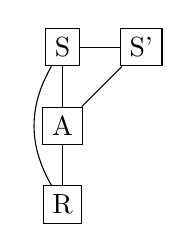
\begin{tikzpicture}[scale=.5,every node/.style={rectangle,draw}]
      \node (n6) at (1,5) {S};
      \node (n4) at (1,3) {A};
      \node (n5) at (3,5) {S'};
      \node (n1) at (1,1) {R};
      \path[every node/.style={font=\sffamily\small}]
      (n6) edge (n4)
      edge (n5)
      edge [bend right] (n1)
      (n4) edge (n1)
      edge (n5);
    \end{tikzpicture}
    \caption{MRF representation of MDP timestep}
    \label{fig:mrf}
  \end{subfigure}
  %add desired spacing between images, e. g. ~, \quad, \qquad etc. 
  %(or a blank line to force the subfigure onto a new line)
  \begin{subfigure}[b]{0.5\textwidth}
    \centering
    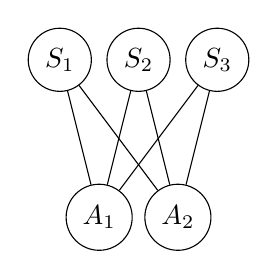
\begin{tikzpicture}[scale=.5,every node/.style={circle,draw}]
      \node (s1) at (1,5) {$S_1$};
      \node (s2) at (3,5) {$S_2$};
      \node (s3) at (5,5) {$S_3$};
      \node (a1) at (2,1) {$A_1$};
      \node (a2) at (4,1) {$A_2$};
      \path[every node/.style={font=\sffamily\small}]
      (s1) edge (a1)
      edge (a2)
      (s2) edge (a1)
      edge (a2)
      (s3) edge (a1)
      edge (a2);
    \end{tikzpicture}
    \caption{MRF sub-node decomposition}
    \label{fig:decomp}
  \end{subfigure}
  \caption{The Markov Decision Process is divided into single timestep experiences each of which can be interpreted as a Markov Random Field by discarding directionality of edges. Each cluster $S,A,R,S'$ may contain many individual nodes. Nodes are fully connected between connected clusters but disconnected within each cluster.}
  \label{fig:structure}
\end{figure}

An exponential family may be defined over the graph in Figure \ref{fig:structure} by introducing potential functions $\phi(X)$ on the nodes and edges. Equation \ref{eqn:exp-family} defines the probability of an assignment $x$ nodes the nodes in the graph given the parameters $\theta$. This is derived from the Potts model described in \cite{wainwright08} using the standard overcomplete representation in which the potential functions $\phi$ take the form of indicator functions over discrete values $\chi$ (Equations \ref{eqn:node-ind}-\ref{eqn:edge-ind}).

\begin{equation}
\label{eqn:exp-family}
p(x;\theta)
=
exp\left\{\sum_{s \in V}\theta_{s;j}(X_s) + \sum_{(s,t) \in E} \theta_{st;jk}(X_s,X_t) - A(\theta)\right\}
\end{equation}

\noindent\begin{minipage}{.4\linewidth}
\begin{equation}
\label{eqn:exp-family}
\theta_{s;j}(X_s) = \sum_{j \in \chi} \theta_{s;j} \mathbb{I}_{s;j}(X_s)
\end{equation}
\end{minipage}%
\begin{minipage}{.6\linewidth}
\begin{equation}
\label{eqn:exp-family}
\theta_{st;jk}(X_s,X_t) = \sum_{jk \in \chi \times \chi} \theta_{st;jk} \mathbb{I}_{st;jk}(X_s,X_t)
\end{equation}
\end{minipage}

\noindent\begin{minipage}{.4\linewidth}
\begin{equation}
\label{eqn:node-ind}
\mathbb{I}_{s;j}(X_s) = \left\{ \begin{array}{rl}
 1 &\mbox{ if $x_s = j$} \\
 0 &\mbox{ otherwise}
\end{array} \right.
\end{equation}
\end{minipage}%
\begin{minipage}{.6\linewidth}
\begin{equation}
\label{eqn:edge-ind}
\mathbb{I}_{st;jk}(X_s,X_t) = \left\{ \begin{array}{rr}
 1 &\mbox{ if $x_s = j, x_t = k$} \\
 0 &\mbox{ otherwise}
\end{array} \right.
\end{equation}
\end{minipage}

\section{Domain}
The experimental domain selected was a 9x9 gridworld pictured in Figure \ref{fig:gridworld}. The gridworld is an MDP in which the agent's state is described by its position (labeled A) in the two-dimensional world and its objective is to reach the goal state (labeled G). The agent takes actions corresponding to movement in any of the four cardinal directions. Each action deterministically moves the agent in the corresponding direction unless the agent has reached the edges of the grid. In this case, no further movement is possible. A reward of 1 is received when the agent reaches the goal state, -1 otherwise.

\begin{figure}
\center
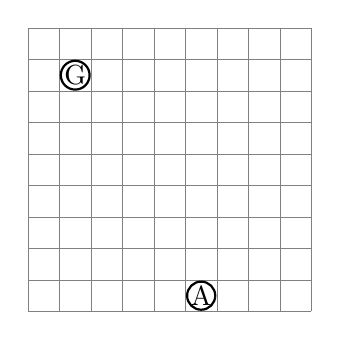
\begin{tikzpicture}[scale=.4,inner sep=0pt,thick,
    dot/.style={fill=blue,circle,minimum size=3pt}]
    \draw[help lines] (0,0) grid (9,9);
    \node[circle,draw] at (5.5,.5) {A};
    \node[circle,draw] at (1.5,7.5) {G};
\end{tikzpicture}
\caption{9x9 Gridworld. A and G respectively represent the agent and goal.}
\label{fig:gridworld}
\end{figure}


\section{Learning Thetas}
Unfortunately, the graph is not triangulated.

\subsection{Pseudo-likelihood Approximation}

\subsection{Automatic Derivation}

\section{Results - Learning}

\section{MAP Inference}

\section{Results - Control}

\section{Future Work}
Learning from more than a single timestep of experience. 
Try out deep learning algorithms on this graph structure.
\section{Discussion and Conclusion}

\bibliography{gm-control}
\bibliographystyle{plain}
\end{document}
